\ifx\mainfile\undefined
%  ========================================================================
%  Copyright (c) 2006-2011 The University of Washington
%
%  Licensed under the Apache License, Version 2.0 (the "License");
%  you may not use this file except in compliance with the License.
%  You may obtain a copy of the License at
%
%      http://www.apache.org/licenses/LICENSE-2.0
%
%  Unless required by applicable law or agreed to in writing, software
%  distributed under the License is distributed on an "AS IS" BASIS,
%  WITHOUT WARRANTIES OR CONDITIONS OF ANY KIND, either express or implied.
%  See the License for the specific language governing permissions and
%  limitations under the License.
%  ========================================================================
%
 
\documentclass [11pt, twoside] {uwthesis}

\usepackage{color}
\usepackage{url}
\usepackage{amsmath}
\usepackage{amsfonts}
\usepackage[bookmarks,
	hidelinks,
	plainpages=false,
	pdfpagelabels,
	pagebackref=true,
            ]{hyperref}
\renewcommand*{\backref}[1]{}% for backref < 1.33 necessary
\renewcommand*{\backrefalt}[4]{%
  \ifcase #1 %
    (No citations.)%
  \or
    (Cited on page #2.)%
  \else
    (Cited on pages #2.)%
  \fi
}

\newcommand{\biburl}[1]{{\tt<}\url{#1}{\tt>}}

\hypersetup{%
pdfauthor = {Daniel Chaim Halperin},
pdftitle = {Simplifying the Configuration of 802.11 Wireless Networks with Effective SNR},
pdfsubject = {Ph.D. Dissertation},
pdfkeywords = {},
pdfcreator = {University of Washington, Computer Science and Engineering},
pdfproducer = {},
bookmarksopen = {true},
pdfpagelayout = {TwoColumnRight},
}

\usepackage{footnotebackref}
%%%%%%%%%%%%%%%%%%%%%%%%%%%%%%%%%%%%%%%%%%%%%%%%%%%%%%
%%%        Formatting sections                     %%%
%%%%%%%%%%%%%%%%%%%%%%%%%%%%%%%%%%%%%%%%%%%%%%%%%%%%%%
\newcommand{\algref}[1]{Algorithm~\ref{#1}}
\newcommand{\chapref}[1]{Chapter~\ref{#1}}
\renewcommand{\eqref}[1]{Equation~\ref{#1}}
\newcommand{\figref}[1]{Figure~\ref{#1}}
\newcommand{\secref}[1]{\S\ref{#1}}
\newcommand{\tabref}[1]{Table~\ref{#1}}
\newcommand{\heading}[1]{\vspace{4pt}\noindent\textbf{#1}}
\newcommand{\topheading}[1]{\noindent\textbf{#1}}
\newcommand{\noheading}[0]{\vspace{4pt}\noindent}

%%%%%%%%%%%%%%%%%%%%%%%%%%%%%%%%%%%%%%%%%%%%%%%%%%%%%%
%%%        XXX and other warnings                  %%%
%%%%%%%%%%%%%%%%%%%%%%%%%%%%%%%%%%%%%%%%%%%%%%%%%%%%%%
\newcommand{\xxx}[1]{\textit{\color{red}XXX #1}}

%%%%%%%%%%%%%%%%%%%%%%%%%%%%%%%%%%%%%%%%%%%%%%%%%%%%%%
%%%        Units                                   %%%
%%%%%%%%%%%%%%%%%%%%%%%%%%%%%%%%%%%%%%%%%%%%%%%%%%%%%%
\usepackage{xspace}
\newcommand{\unitsep}{\texorpdfstring{\,}{ }}
\def\unit#1{% from: http://www.tex.ac.uk/cgi-bin/texfaq2html?label=csname "Defining a macro from an argument"
  \expandafter\def\csname #1\endcsname{\unitsep\text{#1}\xspace}%
}
\def\varunit#1#2{% from: http://www.tex.ac.uk/cgi-bin/texfaq2html?label=csname "Defining a macro from an argument"
  \expandafter\def\csname #1\endcsname{\unitsep\text{#2}\xspace}%
}
\unit{GHz}
\unit{MHz}
\unit{kHz}
\unit{Gbps}
\unit{Mbps}
\unit{KB}
\unit{dB}
\unit{dBi}
\unit{dBm}
\unit{W}
\unit{mW}
\varunit{uW}{$\mu$W}
\unit{ms}
\varunit{us}{$\mu$s}
\unit{h}
\unit{m}
\unit{s}
\unit{km}
\unit{cm}
\unit{mm}
\varunit{mmsq}{mm$^\text{2}$}
\varunit{insq}{in$^\text{2}$}
\newcommand{\degree}{\ensuremath{^\circ}\xspace}
\newcommand{\degrees}{\degree}
%%%%%%%%%%%%%%%%%%%%%%%%%%%%%%%%%%%%%%%%%%%%%%%%%%%%%%%%%%%%%%%%%%%%%%%%%%%%%%%%%%%%%%
% Euler for math | Palatino for rm | Helvetica for ss | Courier for tt
%
% From: http://www.tug.org/mactex/fonts/LaTeX_Preamble-Font_Choices.html
%%%%%%%%%%%%%%%%%%%%%%%%%%%%%%%%%%%%%%%%%%%%%%%%%%%%%%%%%%%%%%%%%%%%%%%%%%%%%%%%%%%%%%
\renewcommand{\rmdefault}{ppl} % rm
\usepackage[scaled]{helvet} % ss
\usepackage{courier} % tt
\usepackage{eulervm} % a better implementation of the euler package (not in gwTeX)
\normalfont
\usepackage[T1]{fontenc}
%%%%%%%%%%%%%%%%%%%%%%%%%%%%%%%%%%%%%%%%%%%%%%%%%%%%%%%%%%%%%%%%%%%%%%%%%%%%%%%%%%%%%%

%%%%%%%%%%%%%%%%%%%%%%%%%%%%%%%%%%%%%%%%%%%%%%%%%%%%%%
%%%        Figures                                 %%%
%%%%%%%%%%%%%%%%%%%%%%%%%%%%%%%%%%%%%%%%%%%%%%%%%%%%%%
\usepackage{graphicx}
% Caption package both lets you set the spacing between figure and caption
% and also makes the \figref{} point to the right place.
\usepackage[font=bf,aboveskip=6pt,belowskip=-4mm]{caption}
% Allow subfigures, make them bold
\usepackage[bf,BF,small]{subfigure}
% List of figures
\setcounter{lofdepth}{2}  % Print the chapter and sections to the lot

%%%%%%%%%%%%%%%%%%%%%%%%%%%%%%%%%%%%%%%%%%%%%%%%%%%%%%
%%%        Lists with reduced spacing              %%%
%%%%%%%%%%%%%%%%%%%%%%%%%%%%%%%%%%%%%%%%%%%%%%%%%%%%%%
\usepackage{enumitem}

%%%%%%%%%%%%%%%%%%%%%%%%%%%%%%%%%%%%%%%%%%%%%%%%%%%%%%
%%%        Fancy tables                            %%%
%%%%%%%%%%%%%%%%%%%%%%%%%%%%%%%%%%%%%%%%%%%%%%%%%%%%%%
\usepackage{tabulary}
\usepackage{booktabs}

%%%%%%%%%%%%%%%%%%%%%%%%%%%%%%%%%%%%%%%%%%%%%%%%%%%%%%
%%%        Formatting techniques/tools/etc.        %%%
%%%%%%%%%%%%%%%%%%%%%%%%%%%%%%%%%%%%%%%%%%%%%%%%%%%%%%
\newcommand{\term}[1]{\texttt{#1}}

\begin{document}
 
\textpages
\setcounter{chapter}{6} % Set to n-1!
\fi
%%%%%%%%%%%%%%%%%%%%%%%%%%%%%%%%%%

\cleardoublepage
\chapter{Application to Rate Selection}
\label{chap:rate}

In the last chapter, I showed that my Effective SNR model can accurately predict packet delivery for 802.11n. Here, I close the loop, demonstrating how my model can be applied to solve an 802.11n configuration problem. This chapter presents an in-depth study of the application of Effective SNR to the problem of rate selection for 802.11.

I first compare against state-of-the-art schemes for single-antenna 802.11a/g systems. In these measurements, the goal is to show that Effective SNR performs as well as or better than the existing, well-studied probe- and channel metric-based schemes on their home ground, using my method which has the advantages of simplicity, deployability, and generality. To enable comparison with state-of-the-art algorithms that cannot be implemented in commodity hardware today, I use 802.11n physical-layer simulations driven by collected channel state information traces to perform my evaluation.

I then show that this model extends well to 802.11n (MIMO) and so provides ongoing value. In subsequent chapters, I will explain how to apply Effective SNR to other configuration problems.

%Rate adaptation is an open problem for 802.11n. Most schemes in the literature were not designed for MIMO systems, and none of the ones that were have been tested on real 802.11 channels.\footnote{The only experimental evaluation of MIMO rate adaptation we know of is on Hydra~\cite{Kim_Hydra}. It uses the USRP radios for 2\MHz channels that are relatively narrowband and flat.} 

\section{Rate Selection Algorithms}
I experiment with ESNR, an algorithm based on my model, plus SampleRate~\cite{Bicket_SampleRate}, the de facto rate selection algorithm in use today, and SoftRate~\cite{Vutukuru_SoftRate}, a research algorithm with the best published results.

\textbf{SampleRate}~\cite{Bicket_SampleRate} is an implicit feedback scheme that uses only information about packet reception or loss.
It maintains delivery statistics for different rates to compute the expected airtime to send a packet, including retries.
It falls back to a lower rate when the airtime of the chosen rate exceeds (due to losses) the airtime of a lower rate.
Standard implementations send a packet to probe 1 or 2 higher rates every 10 packets, to determine whether to switch to higher rates.

The main weakness of SampleRate is its slow reaction to change. If the wireless channel quickly degenerates, SampleRate will incur multiple losses while it falls back through intermediate rates.\footnote{The original SampleRate~\cite{Bicket_SampleRate} did not reduce rate for retries, but some implementations~\cite{Judd_CHARM} and the version used in modern kernels~\cite{Minstrel} do. This turns out to be important for good performance.} When the channel suddenly recovers, SampleRate's infrequent probing converges to the new highest rate slowly. Algorithms such as 
RRAA~\cite{Wong_RRAA} aim to improve on SampleRate's weaknesses, but as they are less widely used we stick with SampleRate as a representative probe-based algorithm.

SampleRate is only defined for SISO links. MIMO breaks some of its assumptions, as higher rates can work when lower ones do not due to different antenna modes. Thus, I only compare it for 802.11a/g experiments.

\textbf{SoftRate}~\cite{Vutukuru_SoftRate} is an explicit feedback scheme that uses information gleaned during packet reception at a given rate to predict how well different rates will work. The input to these predictions is the bit error rate (BER) as estimated from side-information provided by the convolutional decoder. SoftRate chooses rates based on the performance curves that relate the BERs for one rate (a combination of modulation and coding) to another. %the BER for a different modulation and coding. 
Each rate will be the best choice only during a predictable BER range. These predictions can help SoftRate quickly identify the best rate. SoftRate has been shown to dominate trained SNR-based algorithms such as CHARM~\cite{Judd_CHARM} and I do not evaluate against those directly.

%SoftRate drops rate on retries to ensure that packets are delivered.

SoftRate is defined for SISO channels, like SampleRate, 
and its predictions hold only for fixed transmit power and antenna modes, so it does not extend to MIMO systems.
Thus I only use it for 802.11a/g experiments. To cover the full SISO range, I extended the MIT implementation of SoftRate to QAM-64 and 2/3 and 5/6 rate codes.

\textbf{ESNR} uses my model in a very simple way: given recent channel state information, compute the highest rate configuration that is predicted to successfully deliver packets (PRR $>90\%$). It runs at the receiver, measuring CSI on received packets and returning rate changes to the sender along with the ACK like SoftRate. Finally, to protect against poor choices near a rate boundary in our model, I fall back one rate if consecutive packets must be retried and the Effective SNR level has not changed. This is a fixed rule.

Like SoftRate, this algorithm obviates the search phase. There is no calibration of dynamic thresholds. This is not rate \emph{adaptation} so much as rate \emph{selection} that changes only because it tracks the channel's evolution. And unlike SoftRate, the predictions of the model hold over different antenna modes. This lets it run over 802.11n rates as easily and in the same way that it runs over 802.11a/g rates. Thus, I report results from both 802.11a/g and 802.11n runs for this algorithm.

\textbf{Optimal.} I also take advantage of simulation to add upper bounds on achievable performance. This lets me assess how well the algorithms perform on an absolute scale. The OPT scheme has an oracle that knows the true highest rate that can be successfully delivered at any given time. The Previous-OPT scheme knows the optimal rate that worked on the channel for the previous packet and uses it for the next transmission; it just does not know the future. Since SoftRate and ESNR use an estimate of this previous channel state, and SampleRate infers the recent channel state, they are unlikely to beat Previous-OPT. The gap between Previous-OPT and OPT is also likely to be significant because of inherent wireless channel variability.
%OPT gets the benefit of transient improvements and faster rates with low, but non-zero delivery probability for free.


\section{Trace-driven Simulator}

%We use a simulator to compare these algorithms running on the same channel. Our ESNR algorithm runs in real time on a mobile client with the Intel 802.11 NIC\@. However, we turn to simulation for two reasons. First, SoftRate runs on a software-defined radio, not a commercial NIC, so we need to use simulation to compare the two. Second, good algorithms have consistently good performance over a range of channels. For example, no algorithm will beat SampleRate by a significant margin on static channels because it will quickly adapt to the channel. However, algorithms like SoftRate perform well even when the channel is changing rapidly due to mobility. With a simulator, we can compare algorithms over this range of conditions. 

Although the ESNR algorithm runs in real time on a mobile client with the Intel 802.11 NIC,\footnote{I implemented a version of ESNR that randomly probes other antenna modes to collect CSI and that also sends Effective SNR estimates back to the transmitter, and ran it online against SampleRate in human-scale mobility. The results show that the probing and feedback have little penalty, and match the simulator: the two algorithms are separated by a small (5\%--10\%) margin.} I turn to simulations to compare these algorithms. %running on the same channel. 
This is for two reasons. First, SoftRate runs on a software-defined radio, and cannot be implemented on a currently available commercial NIC. Second, U want to compare the algorithms over varied channel conditions, from static to rapidly changing, to assess how consistently they perform. 
For example, no algorithm will beat SampleRate by a significant margin on static channels, because it will eventually adapt to the channel. In contrast, SoftRate performs well even when the channel is changing rapidly due to mobility. However, it is hard to generate controllable high-mobility experimental settings, while traces let us perform these evaluations directly.


%The simulator we build is trace-driven. 

\subsection{Trace} I collected real channel information for the simulations. I walked around UW CSE while carrying a laptop configured to send short, back-to-back packets to stationary testbed nodes that record the CSI. The CSI reflects frequency-selective fading over real, varying 20\MHz MIMO channels that is typically not observed with more narrowband experimentation, e.g., on the USRP. Recall that CSI is estimated during the preamble of the packet transmission, independent of the modulation and coding of the payload. Therefore, the mobile transmitter can quickly cycle through all antenna configurations (SIMO, MIMO2 and MIMO3) by sending a single short UDP packet at the lowest rate for each configuration. This enables fine grained sampling of the channel, approximately every 650\us. The following results are derived from a trace with approximately 85,000 channel measurements taken over 55 seconds, spanning varying RF channels that range from the best 3-stream rates to SISO speeds.

\begin{figure}[ht]
\centering
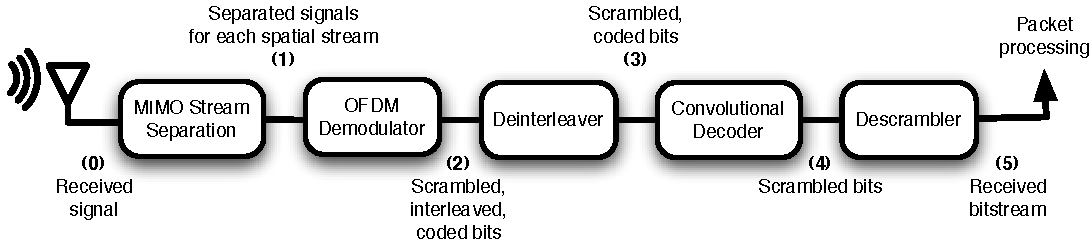
\includegraphics[width=6in]{figures/esnr/mimo_ofdm_decoding_process.pdf}
\caption[The 802.11n MIMO-OFDM decoding process]{\label{fig:ofdm_decoding} The 802.11n MIMO-OFDM decoding process. MIMO receiver separates the RF signal~(0) for each spatial stream~(1). Demodulation converts the separated signals into bits~(2). Bits from the multiple streams are deinterleaved and combined~(3) followed by convolutional decoding~(4) to correct errors. Finally, scrambling that randomizes bit patterns is removed and the packet is processed~(5).}
\end{figure}


\subsection{Simulator} I feed this trace to a custom 802.11a/g/n simulator written in a combination of MATLAB and the MIT C++ GNU Radio code. The simulator implements packet reception as shown in \figref{fig:ofdm_decoding}, including demodulation for BPSK through QAM-64, deinterleaving, and convolutional decoding with soft inputs and soft outputs. The measured CSI is interpolated to 56 carriers and serves as the ground truth for the channel, and packets are correctly received when there are no bit errors, or are lost. SampleRate, SoftRate, and ESNR are implemented as described previously. To ensure that ESNR is not given the unrealistic advantage of ground truth CSI, we corrupt the CSI at the level of ADC quantization, which typically induces an error of $\pm$1.5\dB in the output Effective SNRs. SoftRate estimates the BER directly during decoding.

To vary mobility, we can replay the trace at different speeds. For example, 4$\times$ mobility gives ESNR the CSI from every fourth trace record. However, packet reception still uses all trace records. For a packet to be correctly received in the accelerated trace, it must be received over the intermediate records. The simulator requires correct reception at $\geq$80\% of the records to allow for coding. This models a varying channel that I can only sample for CSI periodically, as happens when CSI is measured during the packet preamble. SoftRate operates using the 80th percentile soft estimate from the range.

The goal is to evaluate the ability of these algorithms to respond to changing channel conditions. Thus, the primary metric is the delivered PHY layer rate per trace index. Higher-layer factors such as MAC backoff, link-layer packet aggregation, and TCP reactions to loss, will affect how this rate translates to throughput.

\begin{figure}[t]
      \centering
      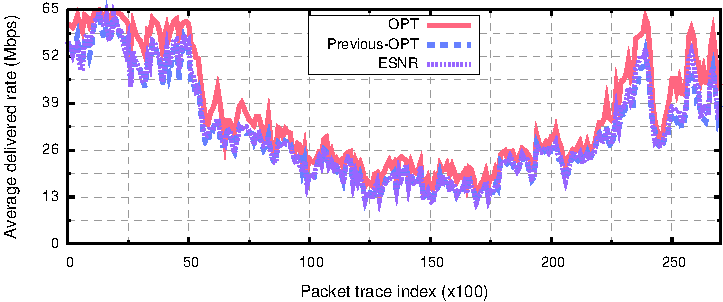
\includegraphics[width=\textwidth]{figures/rate/siso_rate_time_opt_eff.pdf}
      \caption{\label{fig:siso_rate_time_opt_eff} OPT and ESNR SISO performance in human-speed mobility.}
\end{figure}

\begin{figure}[t]
      \centering
      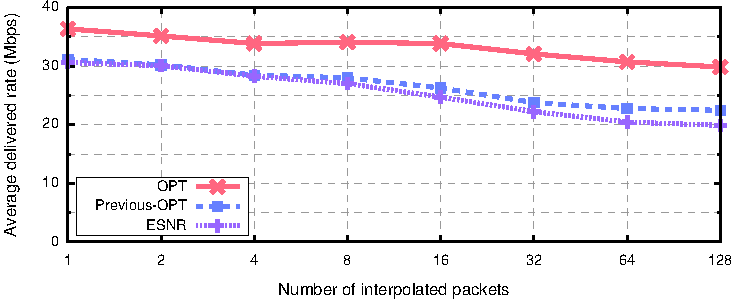
\includegraphics[width=\textwidth]{figures/rate/siso_rate_skip_opt_eff.pdf}
      \caption{\label{fig:siso_rate_skip_opt_eff} OPT and ESNR SISO performance in fast mobile channels.}
\end{figure}



\section{SISO Rate Adaptation Results}
I first examine the performance of ESNR for SISO rates. \figref{fig:siso_rate_time_opt_eff} shows the rate over time for ESNR and OPT over the trace. The performance metric is the average rate over an interval because each algorithm gets an opportunity to send a packet at the same point in the trace. The rate is averaged over a window of 100 packets to smooth the data for readability. ESNR performs excellently. It is below OPT but consistently overlaps Previous-OPT, which is an upper bound for schemes that track the channel and do not predict the future. ESNR is accurate on 75\% of packets, with the expected 10\% target over-selection.

\subsection{Effective SNR vs Optimal}
\figref{fig:siso_rate_skip_opt_eff} shows the effects of mobility on SISO channels. Each line plots the average rate as a function of the speed at which the trace is played. These results cover a large range of speeds to show trends, in doubling increments from 1$\times$ (walking speed, $\approx$3\mph) to 128$\times$ ($>$300\mph). All schemes fall off with increased speed, and the gap between OPT and Previous-OPT grows from 20\% at human speeds to 1/3 at the fastest speeds. However, even in these mobile channels, ESNR holds up very well and tracks Previous-OPT within 10\%.
Note that Packet SNR was observed to fare quite poorly~\cite{Vutukuru_SoftRate} in mobile channels, but since Effective SNR reflects actual link quality its estimates are more accurate (\chapref{chap:delivery}) and stable (2$\times$--3$\times$ less variance).
%Note this is much better than trained SNR techniques~\cite{Vutukuru_SoftRate}, because packet SNR primarily reflects strong subcarriers, while Effective SNR reflects actual performance and is hence more stable.

\begin{figure}[t]
      \centering
      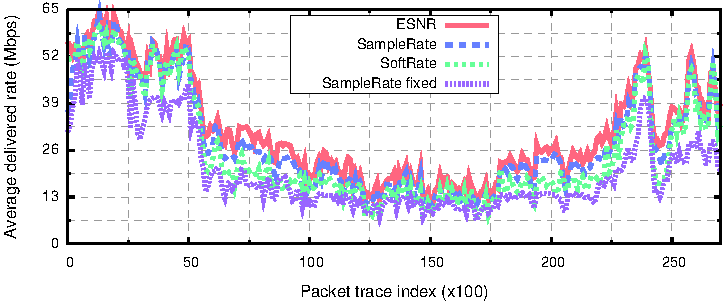
\includegraphics[width=\textwidth]{figures/rate/siso_rate_time_opt_eff_sr_so.pdf}
      \caption{\label{fig:siso_rate_time_opt_eff_sr_so} ESNR, SampleRate, and SoftRate SISO performance in human-speed mobility.}
\end{figure}
\begin{figure}[t]
      \centering
      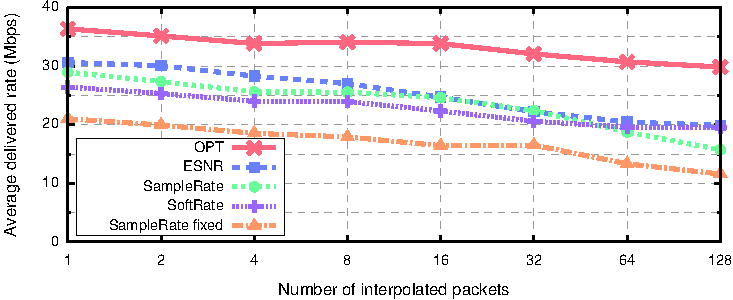
\includegraphics[width=\textwidth]{figures/rate/siso_rate_skip_opt_eff_sr_so.pdf}
      \caption{\label{fig:siso_rate_skip_opt_eff_sr_so} OPT, ESNR, SampleRate, and SoftRate SISO performance in fast mobile channels.}
\end{figure}


\subsection{Effective SNR vs 802.11a/g algorithms}
Next, I compare ESNR with SampleRate and SoftRate. The corresponding rate versus time and rate versus mobility speedup graphs are shown 
in \figref{fig:siso_rate_time_opt_eff_sr_so} and \figref{fig:siso_rate_skip_opt_eff_sr_so}. While it is hard to separate the lines on the graph, at 1$\times$ speed, ESNR slightly outperforms SampleRate which slightly outperforms SoftRate. These results were surprising: SampleRate performs better than expected, and SoftRate performs less well. 


SampleRate's lagging channel estimate makes it degrade fastest with increasing mobility. However, it maintains a 10\%--25\% margin with ESNR, still performing well even with large speedups. In deeper analysis, I discovered that dropping rate on retry is an important factor that gives it short-term adaptability. Without this rate fallback (the ``SampleRate fixed'' line), it loses 25\%--50\% of its performance.

SoftRate has among the slowest falloff with mobility speedup because it directly and accurately measures the channel, and performs the best at maximum speed. However, at slow speeds it is slightly slower on average than SampleRate, though it easily beats a SampleRate without fallback that was the basis for earlier comparisons.\footnote{M. Vutukuru, personal communication, and code inspection.}
This gap is likely not fundamental, as SoftRate's post-decoding BER estimate should match or even slightly improve on ESNR. Further tuning will likely improve SoftRate. Note that the task for SoftRate is harder in our setting than in the original evaluation. I have added QAM-64 and other coding rates, so it must now chose among 8 SISO rates.

Finally, while the performance differences between schemes are significant, they are always less than a factor of two (ignoring OPT). To put this in perspective, note that other evaluations have reported throughput based on TCP traffic, which will magnify performance gaps by reacting to packet loss.

\begin{figure}[t]
      \centering
      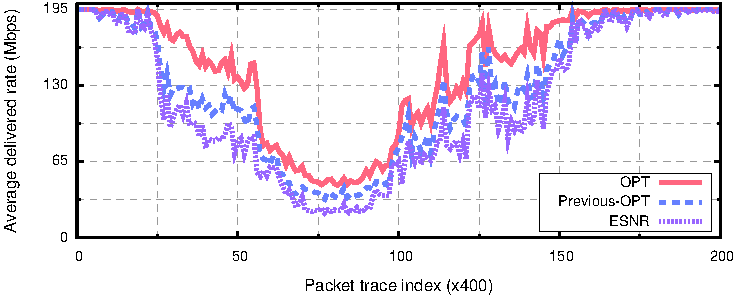
\includegraphics[width=\textwidth]{figures/rate/mimo_skip_time.pdf}
      \caption{\label{fig:mimo_eff_snr_time} OPT and ESNR MIMO performance in human-speed mobility.}
\end{figure}

\begin{figure}[ht]
      \centering
      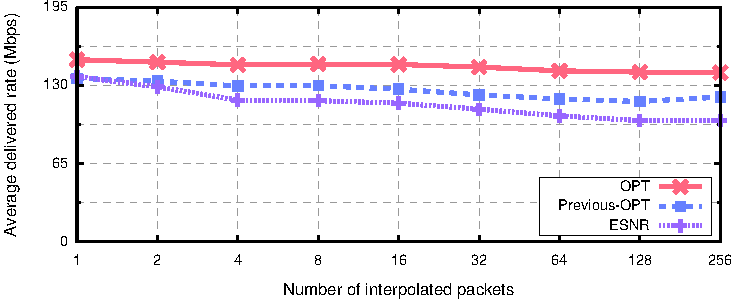
\includegraphics[width=\textwidth]{figures/rate/mimo_rate_skip.pdf}
      \caption{\label{fig:mimo_eff_snr_speedup} OPT and ESNR MIMO performance in faster mobile channels.}
\end{figure}

\section{MIMO Rate Adaptation}
To show the generality of the model, \figref{fig:mimo_eff_snr_time} and \figref{fig:mimo_eff_snr_speedup} show the performance of an unmodified ESNR algorithm running for 802.11n MIMO rates. These results do not include SampleRate or SoftRate as they are SISO schemes. Instead, I use OPT as a benchmark.
%\figref{fig:mimo_eff_snr_time} and \figref{fig:mimo_eff_snr_speedup} show the rate versus time and rate versus speedup graphs. 
These figures are in the same form as for SISO, except the range of rates has grown by a factor of 3 to support up to 195\Mbps. 

The trends in these graphs are similar to those in the SISO graphs: at human mobility speeds, ESNR tracks Previous-OPT and delivers excellent performance, with 80\% accuracy and 10\% over-selection. In faster mobile channels, there is a slightly larger gap with Previous-OPT for MIMO than for SISO, likely because ESNR must now choose between 24 rates instead of 8. It is more likely to choose rates under the highest rate that would have worked. 

Finally, note that with 3 antennas there are only four two- and three-stream rates over 117\Mbps (130, 156, 175.5 and 195 Mbps). The visible gap between indices 25--50 in \figref{fig:mimo_eff_snr_time} reflects only the difference between 1 or 2 rates of potentially different antenna modes. Taken together, these results imply that ESNR's MIMO performance is highly competitive.


\section{Enhancements}
One strength of my model is that it can accommodate choices other than rates. This lets us add other functionality to ESNR without increasing complexity.%We demonstrated an example enhancement to trim excess transmit power in \chapref{chap:delivery}.
% Our example in \secref{sec:delivery} showed that our model has sufficient predictive power to do this. 

\subsection{Transmit antenna selection}
A second enhancement is to select the best transmit antenna when there are spare antennas. %A common scenario is an 802.11n AP sending to an 802.11a/g client. The
An 802.11n AP can select antennas to use to send packets to a legacy 802.11a/g client (plus use all antennas to receive packets). With three antennas to choose from, the expected gain in SNR is a little over 2.5\dB~\cite{Goldsmith}. This is often enough to advance to a higher rate.

I ran a version of SISO ESNR that chose the antenna with the highest ESNR for the next transmission. This gave a gain in the average rate of 5\%.  For comparison, OPT achieved a 10\% increase by always knowing which antenna was best. No other rate adaptation schemes directly support these enhancements.

%%%%%%%%%%%%%%%%%%%%%%%%%%%%%%%%%%
\ifx\mainfile\undefined
%
% ==========   Bibliography   ==========
%
%\nocite{*}   % include everything in the uwthesis.bib file
\bibliographystyle{plain}
\bibliography{dhalperi_thesis}

\end{document}
\fi
